\documentclass{article}

\usepackage{GSReg-style}

\title{GlobalSearchRegression.jl \\
       \vspace{5mm} REPORT} 

%\author{
%  Insert author name \\
%  Insert Institution/Affiliation \\
%  Insert other researcher information \\
%  \texttt{insert@email.com} \\
%   \and if there are more authors
%\author{
%  Insert author name \\
%  insert Institution/Affiliation \\
%  insert other researcher information \\
%  \texttt{insert@email.com} \\
%}

\begin{document}

\maketitle

\vspace{5mm}
\tableofcontents
\clearpage


\section{Introduction}
The advantage of having thousands/millions of features to deal with complex phenomena stimulates an unprecedented number of methodological -and technological- improvements to manage the ‘curse of dimensionality’. 

In Economics, this process has a dual approach with machine-learning (ML) and econometric (EC) algorithms emerging for different purposes: the former for prediction/forecasts (focusing on $\hat{y}$) and the latter for estimation/causal inference (interested in $\hat{\beta}$). Alternatively, the same distinction can be expressed in Diebold’s terms as non-causal vs causal prediction, where ML algorithms are designed to reduce prediction sampling-risks -i.e. learning through cross-validation techniques- and EC methods to identify unbiased multivariate relationships -i.e. avoiding consistency issues through residual and coefficient tests for model selection. 

Following Varian’s advices, about ML and EC complementarities -i.e. merging algorithms from different families to reduce both sampling and model uncertainty-, we are developing a novel multi-layer-multi-algorithm methodology combining two reinforcing paradigms: The London School of Economics (LSE) “Testimation” approach -to obtain information about residual properties- and the Bayesian-like “Double-model averaging” -across different covariates and sub-samples. This methodology includes five complementary layers -handling cross-section, time series and panel data- see \cite{gsreg2019}: 

\begin{enumerate}
    \item Pre-processing: with outlier detection, missing values identification, seasonal adjustment and normalization/standardization functions; 
    
    \item Feature extraction: creation of logs, squares, inverses and interactions from selected variables;
    
    \item Feature pre-selection: using filter and embedded ML algorithms like CFS, Variance threshold and LASSO functions; 
    
    \item Final feature selection: with a modified all-subset regression approach, including residual tests and model averaging capabilities; 
    
    \item Post-estimation fine-tuning: coefficient re-evaluation through cross-validation techniques and model averaging across different k-fold results. 
\end{enumerate}

In order to implement this feature selection algorithm, the following syntax has been used:

\begin{lstlisting} 
  using GlobalSearchRegression
  GlobalSearchRegression.gsr(
    equation = "y x1 x2 x3 x4 x5 x6 x7 x8 x9 x10 x11 x12 x13 x14 x15 x16 x17 x18 x19 x20 x21 x22 x23 x24 x25 x26 x27 x28 x29 x30 x31 x32 x33 x34 x35 x36 x37 x38 x39 x40 x41 x42 x43 x44 x45 x46 x47 x48 x49 x50 x51 x52 x53 x54 x55 x56 x57 x58 x59 x60 x61 x62 x63 x64 x65 x66 x67 x68 x69 x70 x71 x72 x73 x74 x75 x76 x77 x78 x79 x80 x81 x82 x83 x84 x85 x86 x87 x88 x89 x90 x91 x92 x93 x94 x95 x96 x97 x98 x99 x100 x101 x102 x103 x104 x105 x106 x107 x108 x109 x110 x111 x112 x113 x114 x115 x116 x117 x118 x119 x120 x121 x122 x123 x124 x125 x126 x127 x128 x129 x130 x131 x132 x133 x134 x135 x136 x137 x138 x139 x140 x141 x142 x143 x144 x145 x146 x147 x148 x149 x150 x151 x152 x153 x154 x155 x156 x157 x158 x159 x160 x161 x162 x163 x164 x165 x166 x167 x168 x169 x170 x171 x172 x173 x174 x175 x176 x177 x178 x179 x180 x181 x182 x183 x184 x185 x186 x187 x188 x189 x190 x191 x192 x193 x194 x195 x196 x197 x198 x199 x200 x201 x202 x203 x204 x205 x206 x207 x208 x209 x210 x211 x212 x213 x214 x215 x216 x217 x218 x219 x220 x221 x222 x223 x224 x225 x226 x227 x228 x229 x230 x231 x232 x233 x234 x235 x236 x237 x238 x239 x240 x241 x242 x243 x244 x245 x246 x247 x248 x249 x250 x251 x252 x253 x254 x255 x256 x257 x258 x259 x260 x261 x262 x263 x264 x265 x266 x267 x268 x269 x270 x271 x272 x273 x274 x275 x276 x277 x278 x279 x280 x281 x282 x283 x284 x285 x286 x287 x288 x289 x290 x291 x292 x293 x294 x295 x296 x297 x298 x299 x300 x301 x302 x303 x304 x305 x306 x307 x308 x309 x310 x311 x312 x313 x314 x315 x316 x317 x318 x319 x320 x321 x322 x323 x324 x325 x326 x327 x328 x329 x330 x331 x332 x333 x334 x335 x336 x337 x338 x339 x340 x341 x342 x343 x344 x345 x346 x347 x348 x349 x350 x351 x352 x353 x354 x355 x356 x357 x358 x359 x360 x361 x362 x363 x364 x365 x366 x367 x368 x369 x370 x371 x372 x373 x374 x375 x376 x377 x378 x379 x380 x381 x382 x383 x384 x385 x386 x387 x388 x389 x390 x391 x392 x393 x394 x395 x396 x397 x398 x399 x400 x401 x402 x403 x404 x405 x406 x407 x408 x409 x410 x411 x412 x413 x414 x415 x416 x417 x418 x419 x420 x421 x422 x423 x424 x425 x426 x427 x428 x429 x430 x431 x432 x433 x434 x435 x436 x437 x438 x439 x440 x441 x442 x443 x444 x445 x446 x447 x448 x449 x450 x451 x452 x453 x454 x455 x456 x457 x458 x459 x460 x461 x462 x463 x464 x465 x466 x467 x468 x469 x470 x471 x472 x473 x474 x475 x476 x477 x478 x479 x480 x481 x482 x483 x484 x485 x486 x487 x488 x489 x490 x491 x492 x493 x494 x495 x496 x497 x498 x499 x500 x501 x502 x503 x504 x505 x506 x507 x508 x509 x510 x511 x512 x513 x514 x515 x516 x517 x518 x519 x520 x521 x522 x523 x524 x525 x526 x527 x528 x529 x530 x531 x532 x533 x534 x535 x536 x537 x538 x539 x540 x541 x542 x543 x544 x545 x546 x547 x548 x549 x550 x551 x552 x553 x554 x555 x556 x557 x558 x559 x560 x561 x562 x563 x564 x565 x566 x567 x568 x569 x570 x571 x572 x573 x574 x575 x576 x577 x578 x579 x580 x581 x582 x583 x584 x585 x586 x587 x588 x589 x590 x591 x592 x593 x594 x595 x596 x597 x598 x599 x600 x601 x602 x603 x604 x605 x606 x607 x608 x609 x610 x611 x612 x613 x614 x615 x616 x617 x618 x619 x620 x621 x622 x623 x624 x625 x626 x627 x628 x629 x630 x631 x632 x633 x634 x635 x636 x637 x638 x639 x640 x641 x642 x643 x644 x645 x646 x647 x648 x649 x650 x651 x652 x653 x654 x655 x656 x657 x658 x659 x660 x661 x662 x663 x664 x665 x666 x667 x668 x669 x670 x671 x672 x673 x674 x675 x676 x677 x678 x679 x680 x681 x682 x683 x684 x685 x686 x687 x688 x689 x690 x691 x692 x693 x694 x695 x696 x697 x698 x699 x700 x701 x702 x703 x704 x705 x706 x707 x708 x709 x710 x711 x712 x713 x714 x715 x716 x717 x718 x719 x720 x721 x722 x723 x724 x725 x726 x727 x728 x729 x730 x731 x732 x733 x734 x735 x736 x737 x738 x739 x740 x741 x742 x743 x744 x745 x746 x747 x748 x749 x750 x751 x752 x753 x754 x755 x756 x757 x758 x759 x760 x761 x762 x763 x764 x765 x766 x767 x768 x769 x770 x771 x772 x773 x774 x775 x776 x777 x778 x779 x780 x781 x782 x783 x784 x785 x786 x787 x788 x789 x790 x791 x792 x793 x794 x795 x796 x797 x798 x799 x800 x801 x802 x803 x804 x805 x806 x807 x808 x809 x810 x811 x812 x813 x814 x815 x816 x817 x818 x819 x820 x821 x822 x823 x824 x825 x826 x827 x828 x829 x830 x831 x832 x833 x834 x835 x836 x837 x838 x839 x840 x841 x842 x843 x844 x845 x846 x847 x848 x849 x850 x851 x852 x853 x854 x855 x856 x857 x858 x859 x860 x861 x862 x863 x864 x865 x866 x867 x868 x869 x870 x871 x872 x873 x874 x875 x876 x877 x878 x879 x880 x881 x882 x883 x884 x885 x886 x887 x888 x889 x890 x891 x892 x893 x894 x895 x896 x897 x898 x899 x900 x901 x902 x903 x904 x905 x906 x907 x908 x909 x910 x911 x912 x913 x914 x915 x916 x917 x918 x919 x920 x921 x922 x923 x924 x925 x926 x927 x928 x929 x930 x931 x932 x933 x934 x935 x936 x937 x938 x939 x940 x941 x942 x943 x944 x945 x946 x947 x948 x949 x950 x951 x952 x953 x954 x955 x956 x957 x958 x959 x960 x961 x962 x963 x964 x965 x966 x967 x968 x969 x970 x971 x972 x973 x974 x975 x976 x977 x978 x979 x980 x981 x982 x983 x984 x985 x986 x987 x988 x989 x990 x991 x992 x993 x994 x995 x996 x997 x998 x999 x1000",
    data = dataname,
    datanames = [:y, :x1, :x2, :x3, :x4, :x5, :x6, :x7, :x8, :x9, :x10, :x11, :x12, :x13, :x14, :x15, :x16, :x17, :x18, :x19, :x20, :x21, :x22, :x23, :x24, :x25, :x26, :x27, :x28, :x29, :x30, :x31, :x32, :x33, :x34, :x35, :x36, :x37, :x38, :x39, :x40, :x41, :x42, :x43, :x44, :x45, :x46, :x47, :x48, :x49, :x50, :x51, :x52, :x53, :x54, :x55, :x56, :x57, :x58, :x59, :x60, :x61, :x62, :x63, :x64, :x65, :x66, :x67, :x68, :x69, :x70, :x71, :x72, :x73, :x74, :x75, :x76, :x77, :x78, :x79, :x80, :x81, :x82, :x83, :x84, :x85, :x86, :x87, :x88, :x89, :x90, :x91, :x92, :x93, :x94, :x95, :x96, :x97, :x98, :x99, :x100, :x101, :x102, :x103, :x104, :x105, :x106, :x107, :x108, :x109, :x110, :x111, :x112, :x113, :x114, :x115, :x116, :x117, :x118, :x119, :x120, :x121, :x122, :x123, :x124, :x125, :x126, :x127, :x128, :x129, :x130, :x131, :x132, :x133, :x134, :x135, :x136, :x137, :x138, :x139, :x140, :x141, :x142, :x143, :x144, :x145, :x146, :x147, :x148, :x149, :x150, :x151, :x152, :x153, :x154, :x155, :x156, :x157, :x158, :x159, :x160, :x161, :x162, :x163, :x164, :x165, :x166, :x167, :x168, :x169, :x170, :x171, :x172, :x173, :x174, :x175, :x176, :x177, :x178, :x179, :x180, :x181, :x182, :x183, :x184, :x185, :x186, :x187, :x188, :x189, :x190, :x191, :x192, :x193, :x194, :x195, :x196, :x197, :x198, :x199, :x200, :x201, :x202, :x203, :x204, :x205, :x206, :x207, :x208, :x209, :x210, :x211, :x212, :x213, :x214, :x215, :x216, :x217, :x218, :x219, :x220, :x221, :x222, :x223, :x224, :x225, :x226, :x227, :x228, :x229, :x230, :x231, :x232, :x233, :x234, :x235, :x236, :x237, :x238, :x239, :x240, :x241, :x242, :x243, :x244, :x245, :x246, :x247, :x248, :x249, :x250, :x251, :x252, :x253, :x254, :x255, :x256, :x257, :x258, :x259, :x260, :x261, :x262, :x263, :x264, :x265, :x266, :x267, :x268, :x269, :x270, :x271, :x272, :x273, :x274, :x275, :x276, :x277, :x278, :x279, :x280, :x281, :x282, :x283, :x284, :x285, :x286, :x287, :x288, :x289, :x290, :x291, :x292, :x293, :x294, :x295, :x296, :x297, :x298, :x299, :x300, :x301, :x302, :x303, :x304, :x305, :x306, :x307, :x308, :x309, :x310, :x311, :x312, :x313, :x314, :x315, :x316, :x317, :x318, :x319, :x320, :x321, :x322, :x323, :x324, :x325, :x326, :x327, :x328, :x329, :x330, :x331, :x332, :x333, :x334, :x335, :x336, :x337, :x338, :x339, :x340, :x341, :x342, :x343, :x344, :x345, :x346, :x347, :x348, :x349, :x350, :x351, :x352, :x353, :x354, :x355, :x356, :x357, :x358, :x359, :x360, :x361, :x362, :x363, :x364, :x365, :x366, :x367, :x368, :x369, :x370, :x371, :x372, :x373, :x374, :x375, :x376, :x377, :x378, :x379, :x380, :x381, :x382, :x383, :x384, :x385, :x386, :x387, :x388, :x389, :x390, :x391, :x392, :x393, :x394, :x395, :x396, :x397, :x398, :x399, :x400, :x401, :x402, :x403, :x404, :x405, :x406, :x407, :x408, :x409, :x410, :x411, :x412, :x413, :x414, :x415, :x416, :x417, :x418, :x419, :x420, :x421, :x422, :x423, :x424, :x425, :x426, :x427, :x428, :x429, :x430, :x431, :x432, :x433, :x434, :x435, :x436, :x437, :x438, :x439, :x440, :x441, :x442, :x443, :x444, :x445, :x446, :x447, :x448, :x449, :x450, :x451, :x452, :x453, :x454, :x455, :x456, :x457, :x458, :x459, :x460, :x461, :x462, :x463, :x464, :x465, :x466, :x467, :x468, :x469, :x470, :x471, :x472, :x473, :x474, :x475, :x476, :x477, :x478, :x479, :x480, :x481, :x482, :x483, :x484, :x485, :x486, :x487, :x488, :x489, :x490, :x491, :x492, :x493, :x494, :x495, :x496, :x497, :x498, :x499, :x500, :x501, :x502, :x503, :x504, :x505, :x506, :x507, :x508, :x509, :x510, :x511, :x512, :x513, :x514, :x515, :x516, :x517, :x518, :x519, :x520, :x521, :x522, :x523, :x524, :x525, :x526, :x527, :x528, :x529, :x530, :x531, :x532, :x533, :x534, :x535, :x536, :x537, :x538, :x539, :x540, :x541, :x542, :x543, :x544, :x545, :x546, :x547, :x548, :x549, :x550, :x551, :x552, :x553, :x554, :x555, :x556, :x557, :x558, :x559, :x560, :x561, :x562, :x563, :x564, :x565, :x566, :x567, :x568, :x569, :x570, :x571, :x572, :x573, :x574, :x575, :x576, :x577, :x578, :x579, :x580, :x581, :x582, :x583, :x584, :x585, :x586, :x587, :x588, :x589, :x590, :x591, :x592, :x593, :x594, :x595, :x596, :x597, :x598, :x599, :x600, :x601, :x602, :x603, :x604, :x605, :x606, :x607, :x608, :x609, :x610, :x611, :x612, :x613, :x614, :x615, :x616, :x617, :x618, :x619, :x620, :x621, :x622, :x623, :x624, :x625, :x626, :x627, :x628, :x629, :x630, :x631, :x632, :x633, :x634, :x635, :x636, :x637, :x638, :x639, :x640, :x641, :x642, :x643, :x644, :x645, :x646, :x647, :x648, :x649, :x650, :x651, :x652, :x653, :x654, :x655, :x656, :x657, :x658, :x659, :x660, :x661, :x662, :x663, :x664, :x665, :x666, :x667, :x668, :x669, :x670, :x671, :x672, :x673, :x674, :x675, :x676, :x677, :x678, :x679, :x680, :x681, :x682, :x683, :x684, :x685, :x686, :x687, :x688, :x689, :x690, :x691, :x692, :x693, :x694, :x695, :x696, :x697, :x698, :x699, :x700, :x701, :x702, :x703, :x704, :x705, :x706, :x707, :x708, :x709, :x710, :x711, :x712, :x713, :x714, :x715, :x716, :x717, :x718, :x719, :x720, :x721, :x722, :x723, :x724, :x725, :x726, :x727, :x728, :x729, :x730, :x731, :x732, :x733, :x734, :x735, :x736, :x737, :x738, :x739, :x740, :x741, :x742, :x743, :x744, :x745, :x746, :x747, :x748, :x749, :x750, :x751, :x752, :x753, :x754, :x755, :x756, :x757, :x758, :x759, :x760, :x761, :x762, :x763, :x764, :x765, :x766, :x767, :x768, :x769, :x770, :x771, :x772, :x773, :x774, :x775, :x776, :x777, :x778, :x779, :x780, :x781, :x782, :x783, :x784, :x785, :x786, :x787, :x788, :x789, :x790, :x791, :x792, :x793, :x794, :x795, :x796, :x797, :x798, :x799, :x800, :x801, :x802, :x803, :x804, :x805, :x806, :x807, :x808, :x809, :x810, :x811, :x812, :x813, :x814, :x815, :x816, :x817, :x818, :x819, :x820, :x821, :x822, :x823, :x824, :x825, :x826, :x827, :x828, :x829, :x830, :x831, :x832, :x833, :x834, :x835, :x836, :x837, :x838, :x839, :x840, :x841, :x842, :x843, :x844, :x845, :x846, :x847, :x848, :x849, :x850, :x851, :x852, :x853, :x854, :x855, :x856, :x857, :x858, :x859, :x860, :x861, :x862, :x863, :x864, :x865, :x866, :x867, :x868, :x869, :x870, :x871, :x872, :x873, :x874, :x875, :x876, :x877, :x878, :x879, :x880, :x881, :x882, :x883, :x884, :x885, :x886, :x887, :x888, :x889, :x890, :x891, :x892, :x893, :x894, :x895, :x896, :x897, :x898, :x899, :x900, :x901, :x902, :x903, :x904, :x905, :x906, :x907, :x908, :x909, :x910, :x911, :x912, :x913, :x914, :x915, :x916, :x917, :x918, :x919, :x920, :x921, :x922, :x923, :x924, :x925, :x926, :x927, :x928, :x929, :x930, :x931, :x932, :x933, :x934, :x935, :x936, :x937, :x938, :x939, :x940, :x941, :x942, :x943, :x944, :x945, :x946, :x947, :x948, :x949, :x950, :x951, :x952, :x953, :x954, :x955, :x956, :x957, :x958, :x959, :x960, :x961, :x962, :x963, :x964, :x965, :x966, :x967, :x968, :x969, :x970, :x971, :x972, :x973, :x974, :x975, :x976, :x977, :x978, :x979, :x980, :x981, :x982, :x983, :x984, :x985, :x986, :x987, :x988, :x989, :x990, :x991, :x992, :x993, :x994, :x995, :x996, :x997, :x998, :x999, :x1000, :_cons],
    method = :precise,
    intercept = true,
    removeoutliers = ,
    preliminaryselection = :lasso,
    outsample = 10,
    criteria = [:aic, :aicc, :cp, :r2adj, :rmseout],
    ttest = true,
    modelavg = true,
    residualtest = true,
    orderresults = true,
    kfoldcrossvalidation = Dict{Any,Any}(&quot;median&quot;=&gt;[3.0 0.0 0.0 0.0 0.0 0.0 0.0 0.0 0.0 0.0 -0.110223 0.117787 -1.06407 66.0 3.0 56.7211 0.225622 9.63996 0.927044 1.06744 0.201039 0.7426 2.4323e-6 0.655581 0.0 0.0 0.0 0.0 0.0 0.0 0.0 0.0 0.0 0.0 0.0 0.0 0.0 0.0 0.0 0.0 0.0 0.0],&quot;kfolds&quot;=&gt;3,&quot;average&quot;=&gt;[3.33333 0.121148 0.033808 1.19447 -0.135271 0.0442381 -1.01926 0.0 0.0 0.0 -0.102466 0.114535 -0.896072 66.6667 2.66667 55.1408 0.206017 10.058 0.90649 1.1032 0.185638 0.671841 1.62484e-5 0.581203 0.106131 0.0382284 0.925414 0.0920784 0.0328706 0.933747 0.0 0.0 0.0 0.0 0.0 0.0 0.0 0.0 0.0 -0.115661 0.037252 -1.03494],&quot;datanames&quot;=&gt;Symbol[:index, :x6_b, :x6_bstd, :x6_t, :x8_b, :x8_bstd, :x8_t, :x932_b, :x932_bstd, :x932_t, :_cons_b, :_cons_bstd, :_cons_t, :nobs, :ncoef, :sse, :r2, :F, :rmse, :rmseout, :r2adj, :jbtest, :wtest, :order, :x348_b, :x348_bstd, :x348_t, :x806_b, :x806_bstd, :x806_t, :x964_b, :x964_bstd, :x964_t, :x61_b, :x61_bstd, :x61_t, :x428_b, :x428_bstd, :x428_t, :x599_b, :x599_bstd, :x599_t],&quot;tsetsize&quot;=&gt;0.0,&quot;ttest&quot;=&gt;true),
  )
\end{lstlisting}

The report is structured as follows. After this introduction, the methodology is presented. In section 3, descriptive statistics are introduced. After that, LASSO results are examined. Then, All-subset-regression analysis is shown. Finally, the last section examines K-fold cross-validation outcomes.

\section{Methodology}

\subsection{Pre-processing}
It performs required variable transformations to improve model accuracy and feature selection. In this report, it has been used the following internal pre-processing functions:

\begin{enumerate}
  \item Remove-missings: Rows with missing values have been ommited for regression purposes.

  

\end{enumerate}
\subsection{Regularization - LASSO}
The Least Absolute Shrinkage and Selection Operator (LASSO) algorithm is a type of regularized linear regression that uses shrinkage (see \cite{tibshirani1996}) to obtain simple sparse models. This particular type of regression is well-suited for feature selection in models with high levels of muticollinearity, and particularly efficient in fat-data scenarios.

The LASSO regression is a Machine Learning wrapper algorithm (see \cite{chandrashekar2014}) that performs L1 regularization on the optimization function. It adds a penalty term proportional to the sum of coefficients absolute values. With this type of regularization some estimation parameters become zero and -therefore- associated variables can eliminated from the model.
\begin{equation}
    \sum_{n=1}^{n}(y_i - \sum_{j}x_{ij}\beta_{j})^2 + \lambda \sum_{j=1}^p|\beta_{j}|
\end{equation}

Equation (1) entails a residual sum of squares minimization with constraint $\sum \beta_{j}\leq s$. Some of the $\beta_s$ are shrunk to zero, resulting in a more parsimonious regression model.

A tuning parameter, $\lambda$ controls the strength of the L1 penalty. $\lambda$ is basically the amount of shrinkage:

When $ \lambda = 0$, no parameters are eliminated. LASSO estimates replicate OLS ones.

As $\lambda$ increases, more and more coefficients are set to zero and associated variables can be eliminated (theoretically, when $\lambda = \infty$, no covariate is retained).

The choice of $\lambda$ entails a well-known trade-off:  As $\lambda$ increases, estimator bias increases but as $\lambda$ decreases, estimator variance increases (i.e. omitted variables vs model over-fitting).

In this report, the $\lambda$ parameter has been dynamically defined in order to retain up to 3 covariates.

It must be noticed that all predictors are standardized "on-the-fly", in order to avoid scale issues in feature selection.

\subsection{All-subset-Regression}
Unlike other feature selection algorithms (including LASSO), All-subset-regression (ASR) approaches guarantees both in-sample and out-of-sample optimality (i.e. better information criteria results than any other method). However, it has been left aside by econometricians and machine learning practitioners because of computational concerns. Execution times for ASR algorithms in a more-than-20-covariates environement were prohibitive until now. Using existing ASR packages, a simple feature selection problem for 20 covariates usually takes more than 8000 seconds in 
\href{https://cran.r-project.org/web/packages/MuMIn/MuMIn.pdf}{R}, and more than 500000 seconds in \href{https://ideas.repec.org/c/boc/bocode/s457737.html#download}{Stata}. Moreover, with 25 potential covariates both algorithms are unable to obtain feasible-solutions in standard personal computers.

Fortunately, the \verb GlobalSearchRegression.jl package has significantly reduced execution times, running up to 3165 times faster than Stata and 197 times faster than R (see \cite{gsreg2019}). This improvement allows researchers to regain attention on ASR algorithms, looking for better feature selection results. 

In this Julia package, the best model among $2^{n}-1$ alternatives is selected using a potentially composite ordering variable defined as the equally-weighted average of normalized (to guarantee equal weights) and harmonized (to ensure that higher values always identify better models) user's specified criteria. For in-sample adjustment, available alternatives include: Adjusted R2 (:r2adj, the default), Bayesian information criteria (:bic), Akaike and Corrected Akaike information criteria (:aic and :aicc), Mallows's Cp statistic (:cp), Sum of squared errors (also known as Residual sum of squares, :sse) and the Root mean square error (:rmse). For out-of-sample accuracy, there is available the out-of-sample root mean square error (:rmsout). Users are free to combine in-sample and out-of-sample information criteria. In this report, selected information criteria include ([:aic, :aicc, :cp, :r2adj, :rmseout]) as the key variable/s for feature selection.

Additional options applied in this report includes:

\begin{enumerate}
  \item Intercept has been included in all models. Alternatively, users could erase it by selecting the intercept=false boolean option.
  \item The outsample option identifies how many observations are used for prediction purposes. In this case, it has been set to 10.
  \item The user's choice has been ttest=true. Therefore, standard deviation, ttest parameters and related probabilities has been calculated.
  \item Across-models' average coefficients, t-tests and additional statistics were obtained using combined-criteria exponential weights because of the modelavg=true option. More precisely, each alternative model has a weight given by w1/sum(w1), where w1 is defined as exp(-delta/2) and delta is equal to max(index)-index -- where index is the above mentioned normalized, harmonized and potentially combined selection criteria--.
  \item The residualtest=true option enables white heteroskedasticity and Jarque-Bera normality test to be implemented for each model.
  \item The residualtest=true option enables white heteroskedasticity, Jarque-Bera normality test and the Breusch-Godfrey test for autocorrelation to be implemented for each model.
  \item User's specification of orderresults=true entails that the output matrix has been sorted by the the above mentioned normalized, harmonized and potentially combined selection criteria.
\end{enumerate}
\subsection{K-fold Cross Validation}

Cross-validation (CV) is a procedure used to examine feature selection robustness to re-sampling. Among different alternatives, the K-fold approach has a parameter $K$ which identifies the number of groups that a given database must be split into (see \cite{arlot2010}). In this report user selected k-fold number is 3.

The general procedure is as follows:

\begin{enumerate}
  \item Randomly split the database into k disjoint -roughly equally sized- groups
  \item For each group:
  \begin{enumerate}
    \item Take a group as a hold out or test data set (leave-one-out scheme);
    \item Take the remaining groups together as a training data set;
    \item Fit a model on the training set and evaluate it on the test set; and
    \item Retain the evaluation (i.e out-of-sample Root Mean Square Error -RMSE-).
  \end{enumerate}
  \item Summarize model strengths using CV scores
\end{enumerate}

In \verb GlobalSearchRegression.jl  the K-fold cross-validation is available for both LASSO pre-selection and ASR final selection. In the latter, for each K-partition $2^{p} - 1$ alternative models are fitted (where p is the number of potential covariates included in the ASR algorithm) and the candidate ‘optimal’ model is selected using the out-of-sample Root Mean Square Error (obtained from the test set). Therefore, K-candidate models are retained (one for each K-partition). The final "best" model is obtained using either across-model averages or medians. 

This cross-validation specific alternative has been denominated as \textit{Averaging Cross validation (ACV)} by Jung and Hu (see, \cite{jung2015}). The authors found that:

\begin{quote}
"Due to the averaging effect, efficiency of the final parameter estimates obtained by ACV improves over that of the traditional K-fold CV. We note that parameter estimates of CV and ACV are identical when all the candidate ‘optimal’ models from ACV are identical to the model selected by the traditional CV."

\hfill Jung and Hu (2015:168)
\end{quote}

It is worth mentioning that K-fold preferred methodologies change depending on whether cross-section, time-series or panel data observations are employed. For the first one, standard K-fold random allocation is the gold-standard (see \cite{arlot2010}). 

\section{Descriptive Statistics}

Main descriptive statistics for All-subset-regression potential covariates are presented in table 1:

\clearpage

\begin{table}[!h]
  \centering
  \caption{Descriptive Statistics for the main dataset}
    \begin{tabular}{|p{2cm}|p{4cm}|c|c|c|c|c|c|}
    \hline
    Variable & Description & Obs. & Mean & Sd & Max & Min & \% Miss \\
    \hline
    \hline
    x263 & Insert Description & 100 & -0.07 & 1.12 & 2.81 & -2.97 & 0.00\% \\ 
    x779 & Insert Description & 100 & 0.10 & 1.00 & 2.72 & -2.40 & 0.00\% \\ 
    x813 & Insert Description & 100 & -0.02 & 0.88 & 3.64 & -1.77 & 0.00\% \\ 
    \_cons & Insert Description & 100 & 1.00 & 0.00 & 1.00 & 1.00 & 0.00\% \\ 
    \hline
    \end{tabular}
\end{table}

\section{Regularization results}

LASSO regression is shown in the following table:

\begin{table}[!h]
  \centering
  \caption{LASSO Regression results}
    \begin{tabular}{l c}
    \hline
    \hline
              & \\
    Variables & y \\
    \hline
    \hline
      x263 & -0.015 \\
      x779 & -0.005 \\
      x813 & -0.001 \\
    \hline
    \hline
    Observations &  100 \\
    \lambda      &  0.282 \\
    \hline
    \end{tabular}
  \label{tab:addlabel}
\end{table}


\clearpage
\section{Global Search Regression}

\subsection{All sub-subset regression: Best Model and Model Averaging}

\begin{table}[!h]
  \centering
  \caption{GSReg results}
    
    \begin{tabular}{l c c}
    \hline
    \hline
                 &  Best Model               & Model Averaging            \\
    Variables    &  y               & y                 \\
    \hline 
    x263     & -0.253***  & -0.264***     \\
                 & 0.088        & 0.089  \\
     
    x779     & -0.230**  & -0.253**     \\
                 & 0.100        & 0.103  \\
     
    x813     & -0.280**  & -0.299**     \\
                 & 0.115        & 0.118  \\
     
    \_cons     & -0.127  & -0.128     \\
                 & 0.101        & 0.104  \\
    \hline

    Observations &   \multicolumn{ 1  }{c}{ 100 } \\
    Criteria     &   \multicolumn{ 1  }{c}{ [:aic, :aicc, :cp, :r2adj, :rmseout] } \\
    \hline
    \hline
    \multicolumn{ 2  }{c}{Standard errors in parentheses} \\
    \multicolumn{ 2  }{c}{*** p < 0.01, ** p < 0.05, * p < 0.1} \\
    \end{tabular}
  \label{tab:addlabel}
\end{table}

\subsection{Coefficient, t-test and selection criteria gains distributions}

In the following pages, coefficient, t-test and selection criteria distributions are presented. For each covariate, four figures are included: two bivariate density plots (a contour plot and a wireframe plot, for coefficients and t-tests distributions) and two selection criteria contribution plots (a Kernel density plot and a combined Box-Violin plot). The last two plots are used to see the combined\_criteria\_index variation explained by the inclusion of each covariate in the models. 
Finally, we include a unique figure where covariate relative performance is compared using the average impact of each explanatory variable on the combined\_criteria\_index.

\clearpage

\begin{center}
    \large{\textbf{Coefficient, t-test and selection criteria gains distributions for x263 }}
\end{center}

\vspace{-5mm}

\begin{figure}[!ht]
  \centering
  \begin{minipage}[b]{0.46\textwidth}
    \centering
    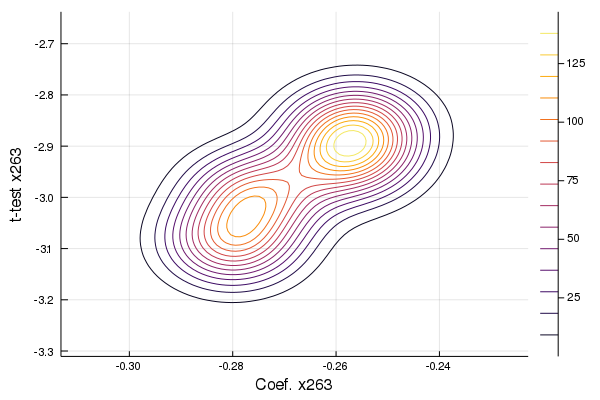
\includegraphics[width=\textwidth]{contour_x263_b_t.png}
    \caption{Bivariate Kernel density (Contour view)}
  \end{minipage}
  \hfill
  \begin{minipage}[b]{0.53\textwidth}
    \centering
    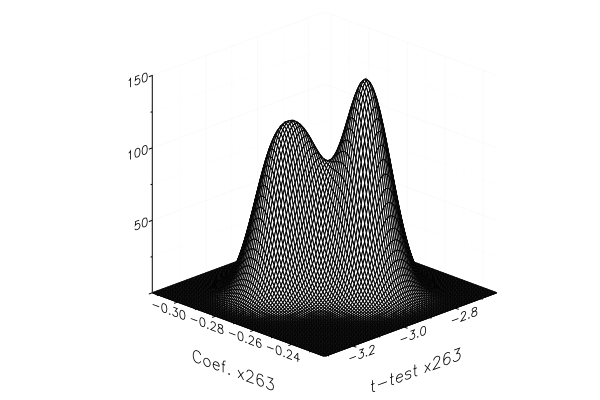
\includegraphics[width=\textwidth]{wireframe_x263_b_t.png}
    \caption{Bivariate Kernel density (Contour view)}
  \end{minipage}

  \begin{minipage}[b]{0.48\textwidth}
    \centering
    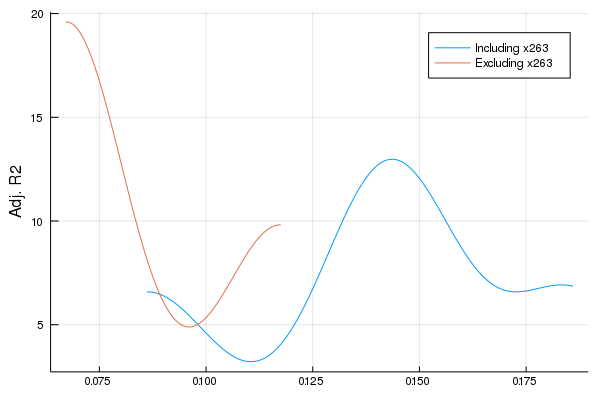
\includegraphics[width=\textwidth]{Kdensity_criteria_x263.png}
    \caption{Selection criteria gains for including x263 (Kernel view)}
  \end{minipage}
  \hfill
  \begin{minipage}[b]{0.48\textwidth}
    \centering    
    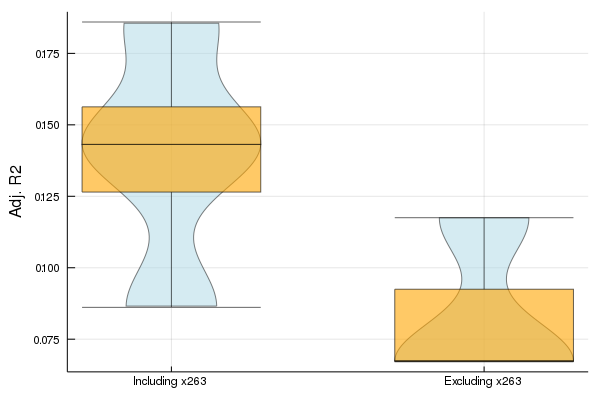
\includegraphics[width=\textwidth]{BoxViolinDot_x263.png}
    \caption{Selection criteria gains for including x263 (Box-Violin view)}    
  \end{minipage}
\end{figure}

\vspace{1cm}

The following table shows main statistics of coefficient and t-test distribution 

\begin{table}[!h]
    \centering
    \caption{Statistics}
    \begin{tabular}{|l|c|c|}
    \hline
    Variable x263 Statistics &  Coefficient Distribution &  T-test Distribution  \\
    \hline
    \hline
    Simple average    & -0.267      & -2.969 \\
    \hline
    Median            & -0.266   & -2.965 \\
    \hline
    Mode              & -0.253     & -2.884 \\
    \hline
    Skewness          & 0.013      & 0.090 \\
    \hline
    kurtosis          & -0.214     & -0.060 \\
    \hline
    Positive Share    & -1.312     & -1.878 \\
    \hline
    Significant Share & 0.000 &  \\
    \hline
    \end{tabular}
\end{table}

\clearpage
\begin{center}
    \large{\textbf{Coefficient, t-test and selection criteria gains distributions for x779 }}
\end{center}

\vspace{-5mm}

\begin{figure}[!ht]
  \centering
  \begin{minipage}[b]{0.46\textwidth}
    \centering
    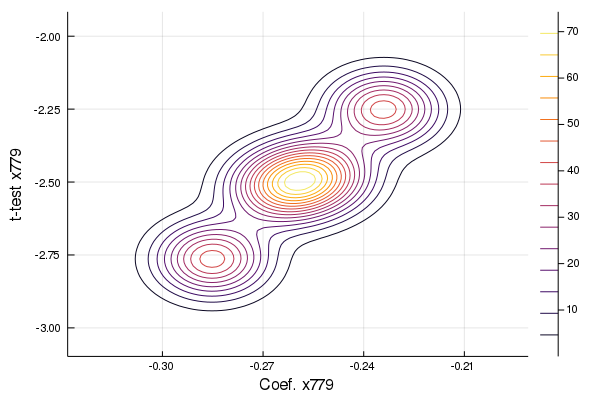
\includegraphics[width=\textwidth]{contour_x779_b_t.png}
    \caption{Bivariate Kernel density (Contour view)}
  \end{minipage}
  \hfill
  \begin{minipage}[b]{0.53\textwidth}
    \centering
    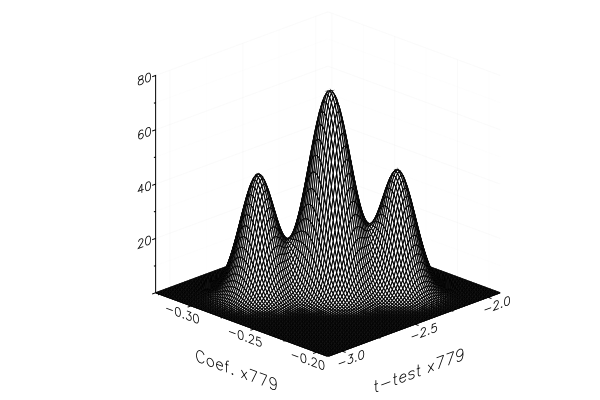
\includegraphics[width=\textwidth]{wireframe_x779_b_t.png}
    \caption{Bivariate Kernel density (Contour view)}
  \end{minipage}

  \begin{minipage}[b]{0.48\textwidth}
    \centering
    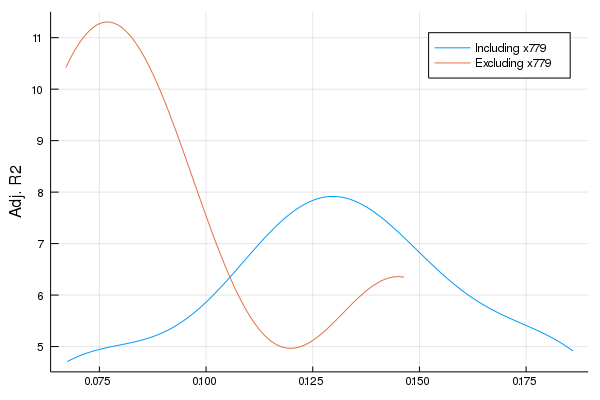
\includegraphics[width=\textwidth]{Kdensity_criteria_x779.png}
    \caption{Selection criteria gains for including x779 (Kernel view)}
  \end{minipage}
  \hfill
  \begin{minipage}[b]{0.48\textwidth}
    \centering    
    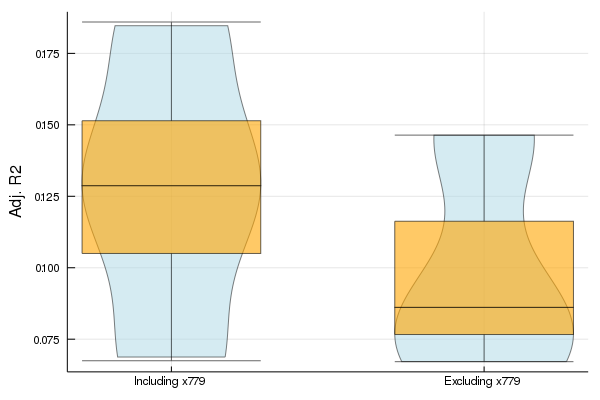
\includegraphics[width=\textwidth]{BoxViolinDot_x779.png}
    \caption{Selection criteria gains for including x779 (Box-Violin view)}    
  \end{minipage}
\end{figure}

\vspace{1cm}

The following table shows main statistics of coefficient and t-test distribution 

\begin{table}[!h]
    \centering
    \caption{Statistics}
    \begin{tabular}{|l|c|c|}
    \hline
    Variable x779 Statistics &  Coefficient Distribution &  T-test Distribution  \\
    \hline
    \hline
    Simple average    & -0.259      & -2.505 \\
    \hline
    Median            & -0.258   & -2.502 \\
    \hline
    Mode              & -0.230     & -2.287 \\
    \hline
    Skewness          & 0.025      & 0.184 \\
    \hline
    kurtosis          & -0.084     & -0.042 \\
    \hline
    Positive Share    & -1.031     & -1.172 \\
    \hline
    Significant Share & 0.000 &  \\
    \hline
    \end{tabular}
\end{table}

\clearpage
\begin{center}
    \large{\textbf{Coefficient, t-test and selection criteria gains distributions for x813 }}
\end{center}

\vspace{-5mm}

\begin{figure}[!ht]
  \centering
  \begin{minipage}[b]{0.46\textwidth}
    \centering
    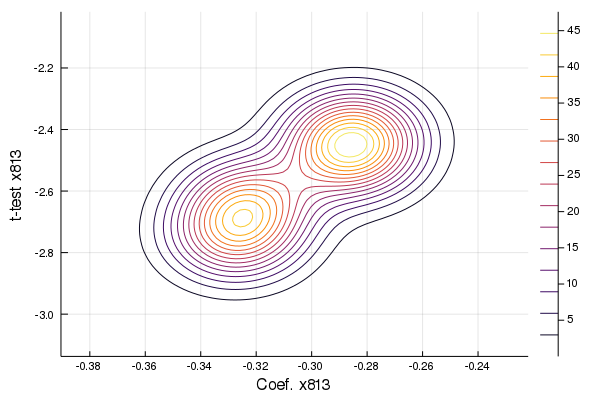
\includegraphics[width=\textwidth]{contour_x813_b_t.png}
    \caption{Bivariate Kernel density (Contour view)}
  \end{minipage}
  \hfill
  \begin{minipage}[b]{0.53\textwidth}
    \centering
    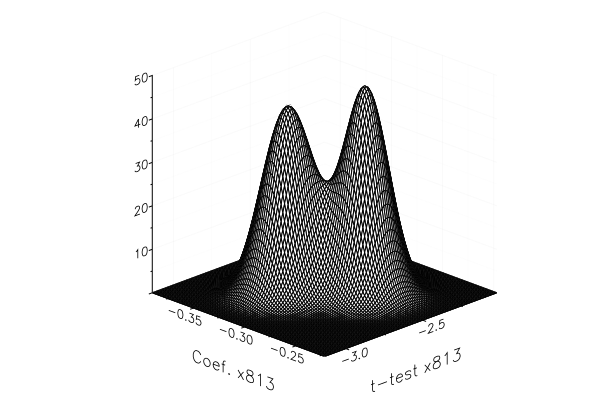
\includegraphics[width=\textwidth]{wireframe_x813_b_t.png}
    \caption{Bivariate Kernel density (Contour view)}
  \end{minipage}

  \begin{minipage}[b]{0.48\textwidth}
    \centering
    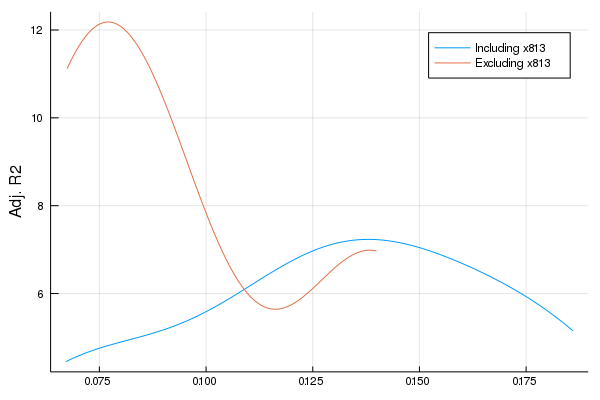
\includegraphics[width=\textwidth]{Kdensity_criteria_x813.png}
    \caption{Selection criteria gains for including x813 (Kernel view)}
  \end{minipage}
  \hfill
  \begin{minipage}[b]{0.48\textwidth}
    \centering    
    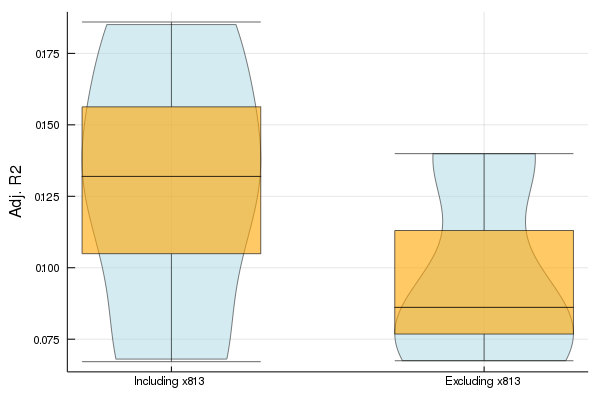
\includegraphics[width=\textwidth]{BoxViolinDot_x813.png}
    \caption{Selection criteria gains for including x813 (Box-Violin view)}    
  \end{minipage}
\end{figure}

\vspace{1cm}

The following table shows main statistics of coefficient and t-test distribution 

\begin{table}[!h]
    \centering
    \caption{Statistics}
    \begin{tabular}{|l|c|c|}
    \hline
    Variable x813 Statistics &  Coefficient Distribution &  T-test Distribution  \\
    \hline
    \hline
    Simple average    & -0.305      & -2.572 \\
    \hline
    Median            & -0.304   & -2.567 \\
    \hline
    Mode              & -0.280     & -2.434 \\
    \hline
    Skewness          & 0.023      & 0.153 \\
    \hline
    kurtosis          & -0.140     & -0.023 \\
    \hline
    Positive Share    & -1.464     & -1.959 \\
    \hline
    Significant Share & 0.000 &  \\
    \hline
    \end{tabular}
\end{table}

\clearpage
\begin{center}
    \large{\textbf{Coefficient, t-test and selection criteria gains distributions for _cons }}
\end{center}

\vspace{-5mm}

\begin{figure}[!ht]
  \centering
  \begin{minipage}[b]{0.46\textwidth}
    \centering
    \includegraphics[width=\textwidth]{contour__cons_b_t.png}
    \caption{Bivariate Kernel density (Contour view)}
  \end{minipage}
  \hfill
  \begin{minipage}[b]{0.53\textwidth}
    \centering
    \includegraphics[width=\textwidth]{wireframe__cons_b_t.png}
    \caption{Bivariate Kernel density (Contour view)}
  \end{minipage}

  \begin{minipage}[b]{0.48\textwidth}
    \centering
    \includegraphics[width=\textwidth]{Kdensity_criteria__cons.png}
    \caption{Selection criteria gains for including _cons (Kernel view)}
  \end{minipage}
  \hfill
  \begin{minipage}[b]{0.48\textwidth}
    \centering    
    \includegraphics[width=\textwidth]{BoxViolinDot__cons.png}
    \caption{Selection criteria gains for including _cons (Box-Violin view)}    
  \end{minipage}
\end{figure}

\vspace{1cm}

The following table shows main statistics of coefficient and t-test distribution 

\begin{table}[!h]
    \centering
    \caption{Statistics}
    \begin{tabular}{|l|c|c|}
    \hline
    Variable _cons Statistics &  Coefficient Distribution &  T-test Distribution  \\
    \hline
    \hline
    Simple average    & -0.128      & -1.223 \\
    \hline
    Median            & -0.127   & -1.244 \\
    \hline
    Mode              & -0.127     & -1.263 \\
    \hline
    Skewness          & 0.018      & 0.180 \\
    \hline
    kurtosis          & 0.016     & 0.125 \\
    \hline
    Positive Share    & -1.293     & -1.131 \\
    \hline
    Significant Share & 0.000 &  \\
    \hline
    \end{tabular}
\end{table}

\clearpage

\begin{figure}[!ht]
    \centering
    \caption{Covariable relevance related to selection criteria}
    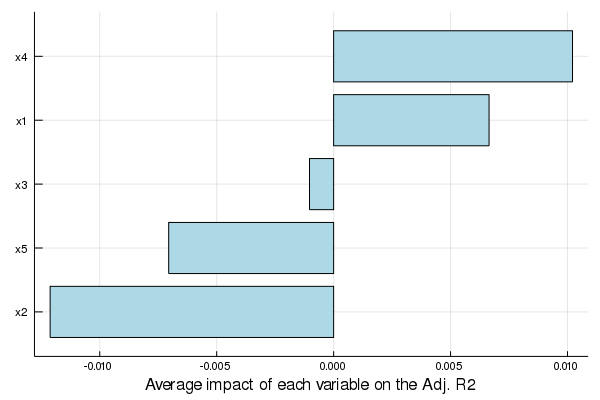
\includegraphics[scale=0.6]{cov_relevance.png}
\end{figure}

%In this figure it is shown that potential covariates included in the general unrrestricted model of the all-subset-regression algorithm display singnificant differences in terms of the user selected information criteria. For each explanatory variable information criteria gains were obtained as the differece between averages information criteria obtained from models which includes and excludes that covariate. Available statistics suggests that there   explanatory  that improved model accuracy.  or }} helps to increase up to a \% the user selected information criteria. On the contrary, there    that have a deleterious impact on model accuracy. This is specially true for , which seems to decrease up to a \% the user selected information criteria}}

\section{k-fold cross-validation}

\begin{table}[!h]
  \centering
  \caption{K-fold cross-validation Results}
    \begin{tabular}{l c c}
    \hline
    \multicolumn{3}{c}{K-fold scheme:\textbf{Insert scheme}}    \\
                    & 3-fold         & 3-fold \\
    Variables       & Mean                    & Median          \\
    \hline
    \hline
[3.0 0.0 0.0 0.0 0.0 0.0 0.0 0.0 0.0 0.0 -0.110223 0.117787 -1.06407 66.0 3.0 56.7211 0.225622 9.63996 0.927044 1.06744 0.201039 0.7426 2.4323e-6 0.655581 0.0 0.0 0.0 0.0 0.0 0.0 0.0 0.0 0.0 0.0 0.0 0.0 0.0 0.0 0.0 0.0 0.0 0.0]

--


[3.33333 0.121148 0.033808 1.19447 -0.135271 0.0442381 -1.01926 0.0 0.0 0.0 -0.102466 0.114535 -0.896072 66.6667 2.66667 55.1408 0.206017 10.058 0.90649 1.1032 0.185638 0.671841 1.62484e-5 0.581203 0.106131 0.0382284 0.925414 0.0920784 0.0328706 0.933747 0.0 0.0 0.0 0.0 0.0 0.0 0.0 0.0 0.0 -0.115661 0.037252 -1.03494]

    \hline

    Error out-sample &     &   \\
                     &     &   \\
    \hline
    \hline
    \multicolumn{3}{c}{\textit{Standard errors in parentheses}} \\
    \multicolumn{3}{c}{*** p < 0.01, ** p < 0.05, * p < 0.1} \\
    \hline
    \end{tabular}
  \label{tab:addlabel}
\end{table}

\addcontentsline{toc}{section}{References} 
\bibliographystyle{unsrt}  
\begin{thebibliography}{1}

\bibitem{gsreg2019}
Panigo D., Glüzmann P., Mocskos, E., Mauri Ungaro, A., Mari, V., and Monzón, N. (2019). \textit{GlobalSearchRegression.jl: Building bridges between Machine Learning and Econometrics in Fat-Data scenarios}.Paper presented at JuliaCon2019, Baltimore-MD, United States.

\bibitem{hassani2007}
Hassani H. (2007). \textit{Singular Spectrum Analysis: Methodology and Comparison}. Journal of Data Science, 5, 239-257.

\bibitem{lehmann2013}
Lehmann, R. (2013). \textit{3 sigma-rule for outlier detection from the viewpoint of geodetic adjustment}. Journal of Surveying Engineering, 139(4), 157-165.

\bibitem{tibshirani1996}
Tibshirani, R. (1996). \textit{Regression shrinkage and selection via the lasso}. Journal of the Royal Statistical Society: Series B (Methodological), 58(1), 267-288.

\bibitem{chandrashekar2014}
Chandrashekar, G., and Sahin, F. (2014). \textit{A survey on feature selection methods}. Computers & Electrical Engineering, 40(1), 16-28.

\bibitem{gluzmann2015}
Gluzmann, P., and Panigo, D. (2015). \textit{Global search regression: A new automatic model-selection technique for cross-section, time-series, and panel-data regressions.} The Stata Journal, 15(2), 325-349.

\bibitem{arlot2010}
Arlot, S., and Celisse, A. (2010).\textit{A survey of cross-validation procedures for model selection}. Statistics surveys, 4, 40-79.

\bibitem{jung2015}
Jung, Y., and Hu, J. (2015). \textit{A K-fold averaging cross-validation procedure}. Journal of nonparametric statistics, 27(2), 167-179.

\bibitem{bergmeir2012}
Bergmeir, C., and Benítez, J. M. (2012). \textit{On the use of cross-validation for time series predictor evaluation}. Information Sciences, 191, 192-213.

\bibitem{bergmeir2018}
Bergmeir, C., Hyndman, R. J., and Koo, B. (2018). \textit{A note on the validity of cross-validation for evaluating autoregressive time series prediction}. Computational Statistics & Data Analysis, 120, 70-83.

\bibitem{hyndman2013}
Hyndman, R. J., and Athanasopoulos, G. (2013). Measuring forecast accuracy. Gilliland M, Tashman L, Sglavo U. Business forecasting: practical problems and solutions, 177-84.

\end{thebibliography}


\end{document}